\section{Description détaillée du nouveau logiciel}
\paragraph{}
Dans cette partie, nous allons explorer la mécanique interne du programme VisualImpro, tout d'abord de façon générale, puis nous allons entrer en détail dans les composantes principales de ce programme, afin que l'on puisse avoir une vision d'ensemble claire et précise des fonctionnalités. 
\subsection{Le point d'entrée du programme}
\paragraph{}
Lorsque le programme est lancé via l'éxécutable, il se passe alors plusieurs choses :
\begin{itemize}
    \item Les paramètres sont chargés sur Bela à travers un fichier de configuration. Ce fichier contient les différentes entrées (audio, analogiques ou fichiers \verb!.wav!) que Bela va traiter ainsi que les différents traitements qui seront appliqués à ces entrées. 
    \item Si des fichiers \verb!.wav! sont indiqués dans le fichier de configuration, alors ceux ci seront aussi chargés sur Bela.
\end{itemize}
\paragraph{}
Ensuite, le programme VisualImpro de Bela débute. La première tâche effectuée par la fonction \verb!main()! est de récupérer le fichier de configuration et de stocker les divers paramètres écrits à l'intérieur de celui-ci. Puis à l'aide des différents paramètres, la deuxième tâche de la fonction \verb!main()!
va être d'initialiser les éléments correspondants. Enfin, la dernière tâche de la fonction \verb!main()! va être de donner la main à la fonction principale de traitement audio à travers l'appel \verb!Bela_startAudio()!. Avec cet appel, on passe à la fonction principale qui se situe dans le fichier \verb!render.cpp! et qui porte le nom de \verb!render()!.
\subsection{La boucle de traitement principale}
\paragraph{}
Avant de passer directement à la fonction \verb!render()!, le programme va passer par la fonction \verb!setup()! qui va initialiser toutes les structures nécessaires au bon déroulement de la fonction \verb!render()!, ainsi qu'un autre élément central du programme, les tâches auxiliaires. Ces tâches auxiliaires, qui font partie des éléments fournis par le framework Bela, permettent au programmeur de créer des segments de code qui seront exécutés en parallèle, ce qui permet d'alléger le travail effectué dans la fonction \verb!render()!, et donc d'éviter de créer des latences qui pourraient perturber le retour en temps réel. C'est pour cela que l'on initialise des tâches auxiliaires dans la fonction \verb!setup()! en spécifiant le code qui sera éxécuté dans chacune d'entre elles. Parmi les 3 différentes tâches présentes dans le code, seules 2 sont intéressantes : la tâche qui aura pour but de remplir les tampons, et celle qui traitera un tampon rempli. La troisième consiste à appliquer des effets sur un tampon, mais ce n'est pas un aspect du projet qui sera traité.
\paragraph{}
Par la suite, la fonction principale \verb!render()! va être appelée en chaîne, jusqu'à ce qu'un signal lui indique qu'elle peut s'arrêter. Dans cette fonction, il va se passer plusieurs choses : 
\begin{itemize}
    \item Si les différents tampons ne sont pas tous remplis, alors on déclenche la tâche auxiliaire de remplissage,
    \item Une fois que les tampons sont remplis, on déclenche la tâche auxiliaire de traitement,
    \item Enfin, on récupère les signaux après traitement et on les envoie sur la sortie audio de Bela.
\end{itemize}
\begin{figure}[H]
    \centering
    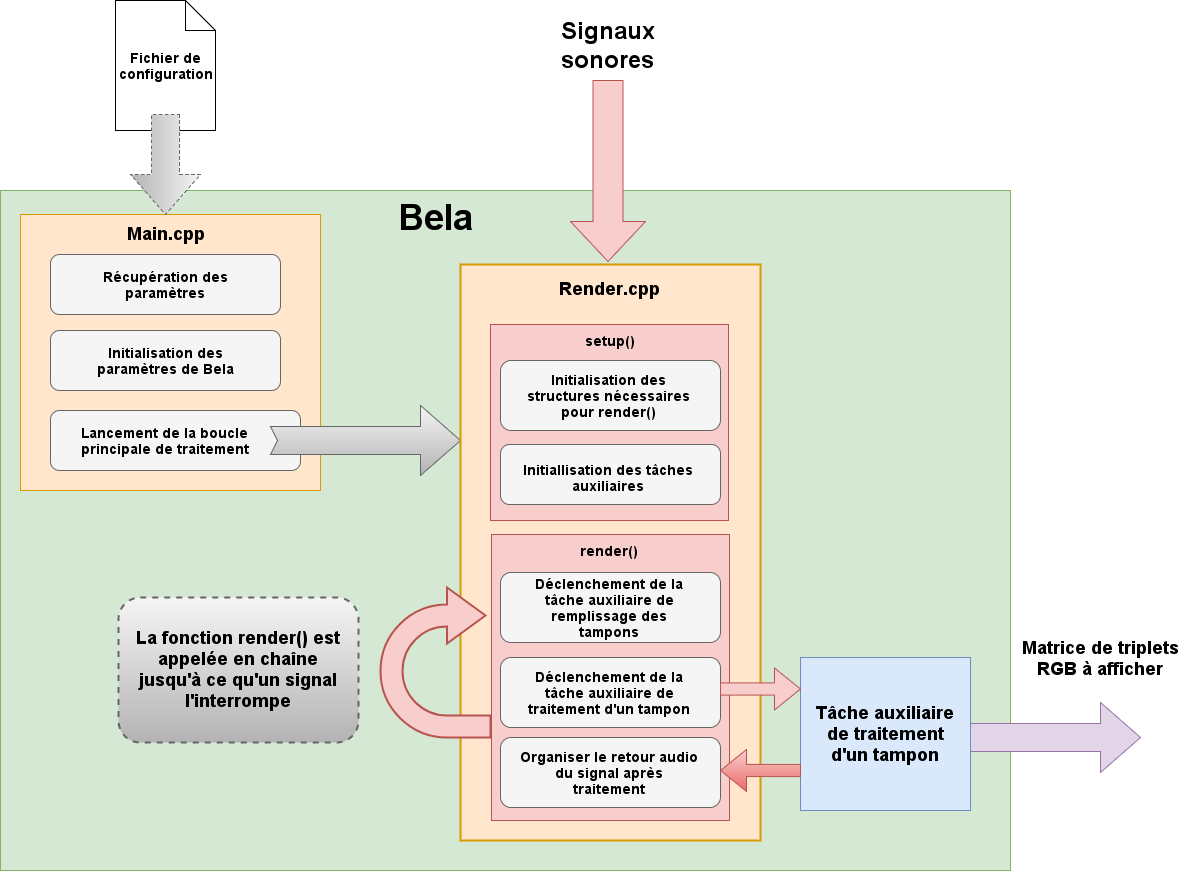
\includegraphics[scale=0.4]{assets/render.png}
    \caption{Fonctionnement des fonctions principales de l'outil}
    \label{focntionnement main render}
\end{figure}